\begin{figure*}[ht]
\centering
\begin{minipage}{0.9\textwidth}
\centering
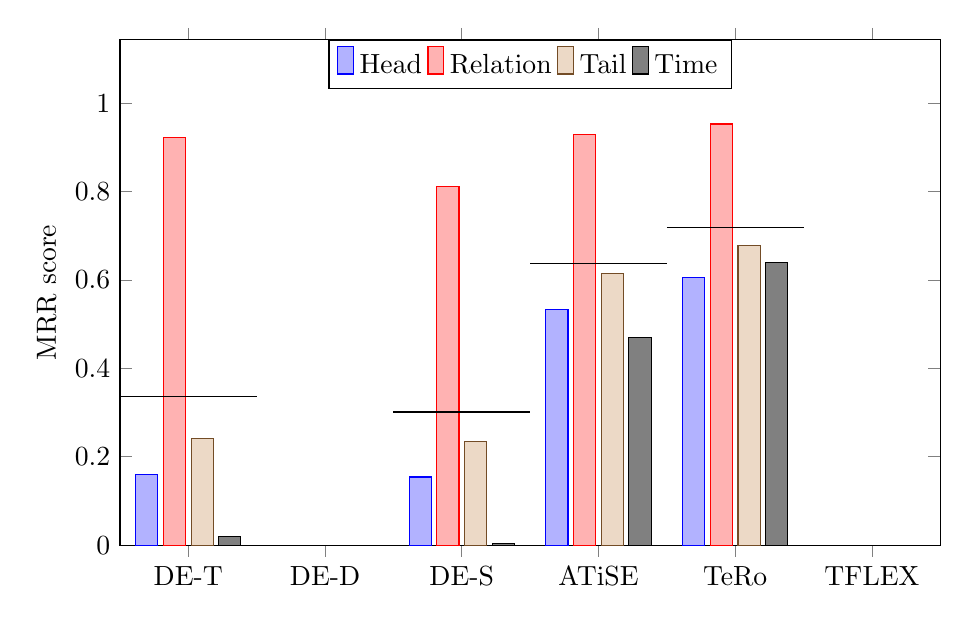
\begin{tikzpicture}
\begin{axis}[
    ybar,
    bar width=8pt,
    xticklabels={x,DE-T,DE-D,DE-S,ATiSE,TeRo,TFLEX},
    ymin=0,
    ymax=1.1435875200261874,
    ylabel={MRR score},
    height=8cm,
    width=12cm,
    legend style={
        at={(0.5,1.0)},
        anchor=north,
        legend columns=-1
    },
    legend image code/.code={
        \draw [#1] (0cm,-0.1cm) rectangle (0.2cm,0.25cm); },
    ]
\addplot coordinates { %head
(0, 0.1600322415080232) %DE_TransE
(1, 0) %DE_DistMult
(2, 0.15417392324803428) %DE_SimplE
(3, 0.5337434445473753) %ATISE
(4, 0.6058347902914908) %TERO
(5, 0) %TFLEX
} ;
\addplot coordinates { %relation
(0, 0.9218881599136685) %DE_TransE
(1, 0) %DE_DistMult
(2, 0.8120719789834734) %DE_SimplE
(3, 0.9300308442835398) %ATISE
(4, 0.9529896000218229) %TERO
(5, 0) %TFLEX
} ;
\addplot coordinates { %tail
(0, 0.24173852707237695) %DE_TransE
(1, 0) %DE_DistMult
(2, 0.23466032281672947) %DE_SimplE
(3, 0.6144979850712404) %ATISE
(4, 0.6780971226548503) %TERO
(5, 0) %TFLEX
} ;
\addplot coordinates { %time_from
(0, 0.020091757176631874) %DE_TransE
(1, 0) %DE_DistMult
(2, 0.0046233366409017046) %DE_SimplE
(3, 0.46980049178075195) %ATISE
(4, 0.6388898627366323) %TERO
(5, 0) %TFLEX
} ;
\addplot[black,sharp plot,update limits=false,] coordinates { %DE_TransE
(-0.5, 0.33593767141767117)
(0.5, 0.33593767141767117)
} ;
\addplot[black,sharp plot,update limits=false,] coordinates { %DE_DistMult
(0.5, 0)
(1.5, 0)
} ;
\addplot[black,sharp plot,update limits=false,] coordinates { %DE_SimplE
(1.5, 0.30138239042228165)
(2.5, 0.30138239042228165)
} ;
\addplot[black,sharp plot,update limits=false,] coordinates { %ATISE
(2.5, 0.6370181914207451)
(3.5, 0.6370181914207451)
} ;
\addplot[black,sharp plot,update limits=false,] coordinates { %TERO
(3.5, 0.7189528439262118)
(4.5, 0.7189528439262118)
} ;
\addplot[black,sharp plot,update limits=false,] coordinates { %TFLEX
(4.5, 0)
(5.5, 0)
} ;
\legend{Head,Relation,Tail,Time}
\end{axis}
\end{tikzpicture}
\caption{wikidata12k, split 1}
\label{fig:compare_wikidata12k_1}
\end{minipage}
\end{figure*}
